% DESCRIBE BRIEFLY THE HAND

There are several ways to implement underactuation in a dexterous hand. In this paper we employ an approach based on adaptive synergy transmission, due to its simplicity and robust design, and its ability for complex interaction with the environment. The Pisa/IIT SoftHand~\cite{Catalano2014Adaptive} implements such a transmission mechanism. This hand has 19 degrees of freedom (DoF) distributed over four fingers and an opposable thumb, but only 1 degree of actuation (DoA). The synergy motion of the hand in free space has been derived from databases of human hand postures. The overall behaviour parameters are the matrices that correspond to the transmission ratio,~$R$, to the joint stiffness,~$K_q$. The actuation is done through a single tendon routed throuh all joints, making the fingers flex and abduct.

% THE LACK OF SENSORS AND FUTURE LARGE DATASETS REQUIRED JUSTIFY THE USE OF SIMULATED DATA

Moving such a hand to grasp an object results in a hard-to-predict contact and hand shapes due to the adaptivity. We thus generate a variety of grasp examples to cover a portion of the interaction space. However, recording many trajectories of all the finger elements that affect the grasp in the real world is non-trivial. For this reason, we generate the example interactions for training using a rigid-body physics simulator, where these problems are avoided. The main two simulation elements we have developed are the contact stability model and the hand behavior model. In the case of the Pisa/IIT softhand, the latter depends heavily on the former. We used the standard distribution of Gazebo and Open Dynamic Engine, both in widespread use. The adaptive synergy equations have been implemented as a plugin to these, and accompany the proper kinematic description of the Pisa/IIT SoftHand\footnote{The Pisa/IIT SoftHand ROS/Gazebo packages are available at \url{https://github.com/CentroEPiaggio/pisa-iit-soft-hand}}.

\begin{figure}
  \centering
  \begin{tabular}{ccc}

  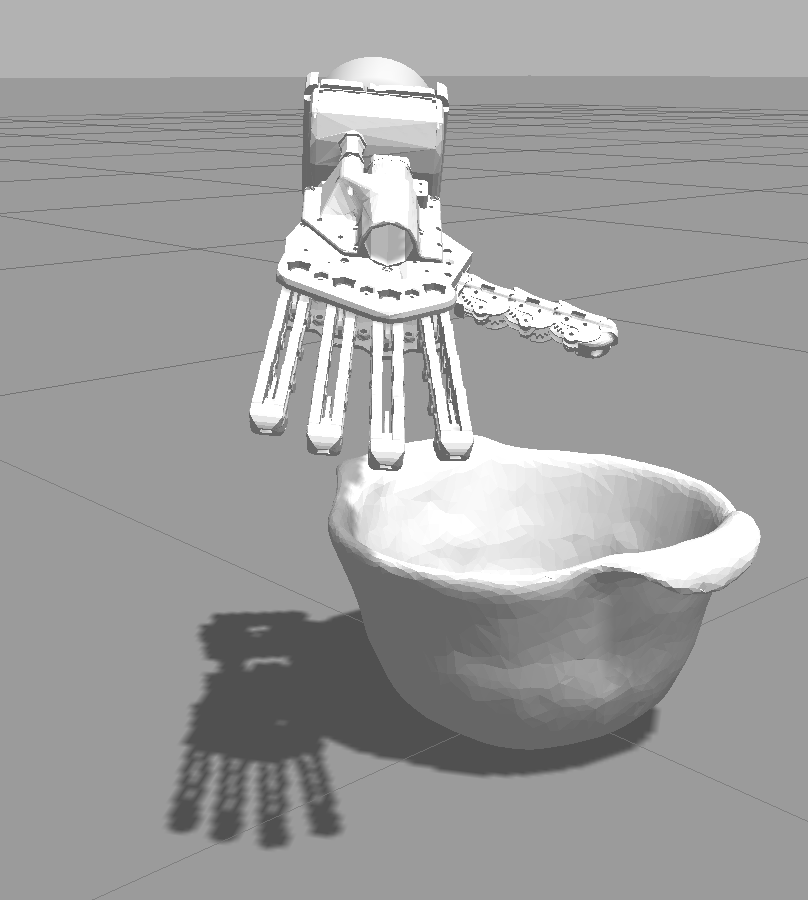
\includegraphics[width=0.3\linewidth]{containerB_pinch_1.png} &

  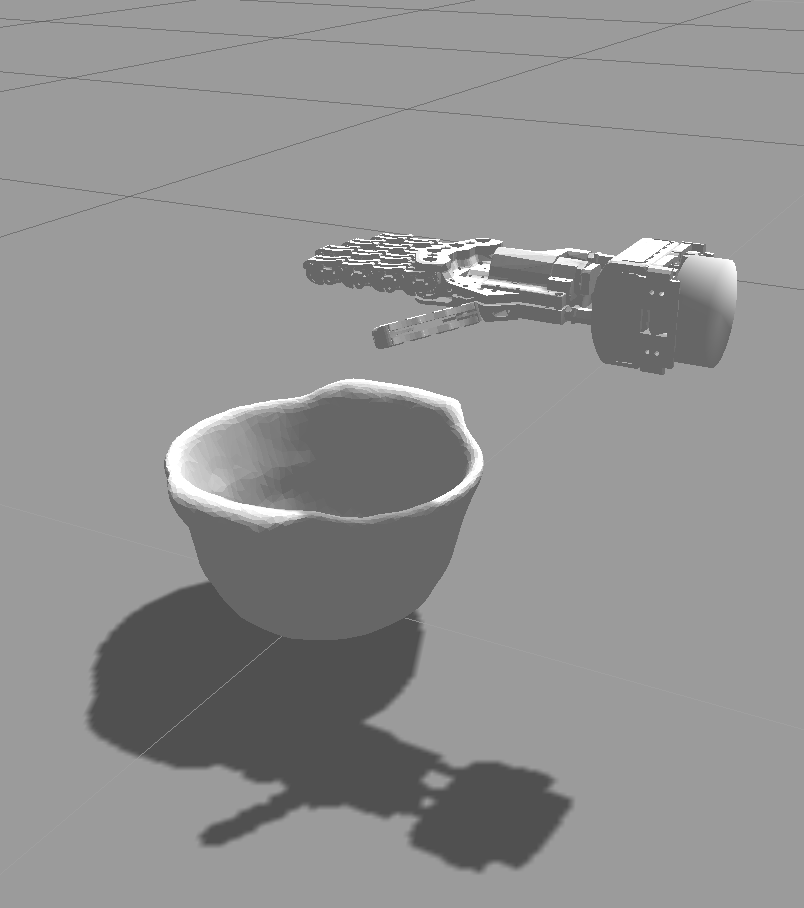
\includegraphics[width=0.3\linewidth]{containerB_rim_1.png} &

  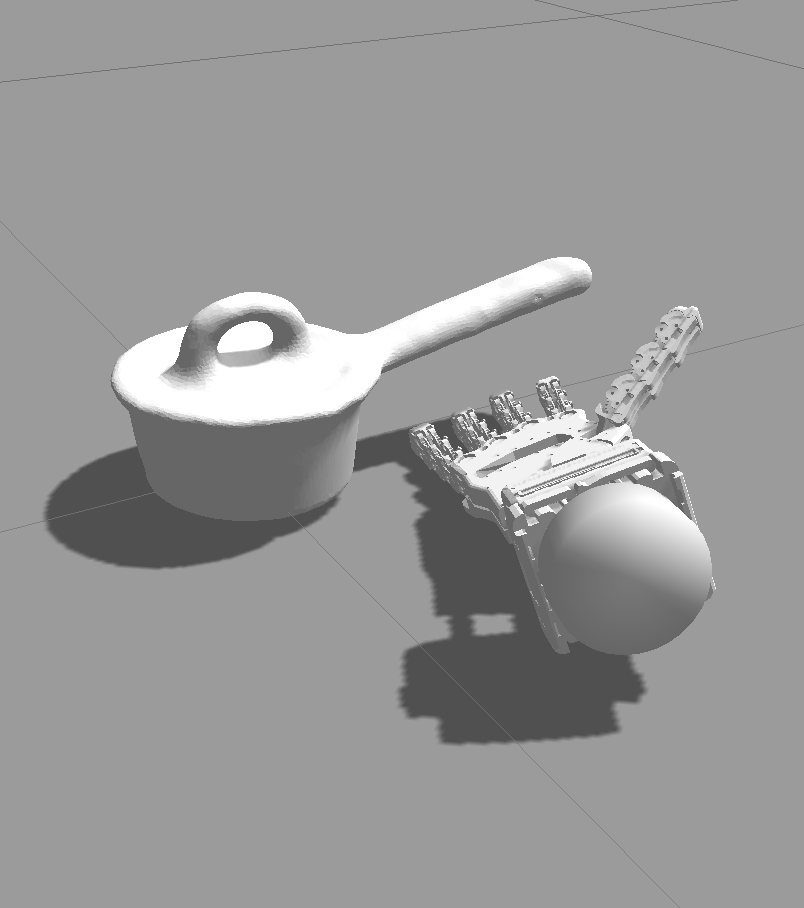
\includegraphics[width=0.3\linewidth]{pot_1.png} \\

  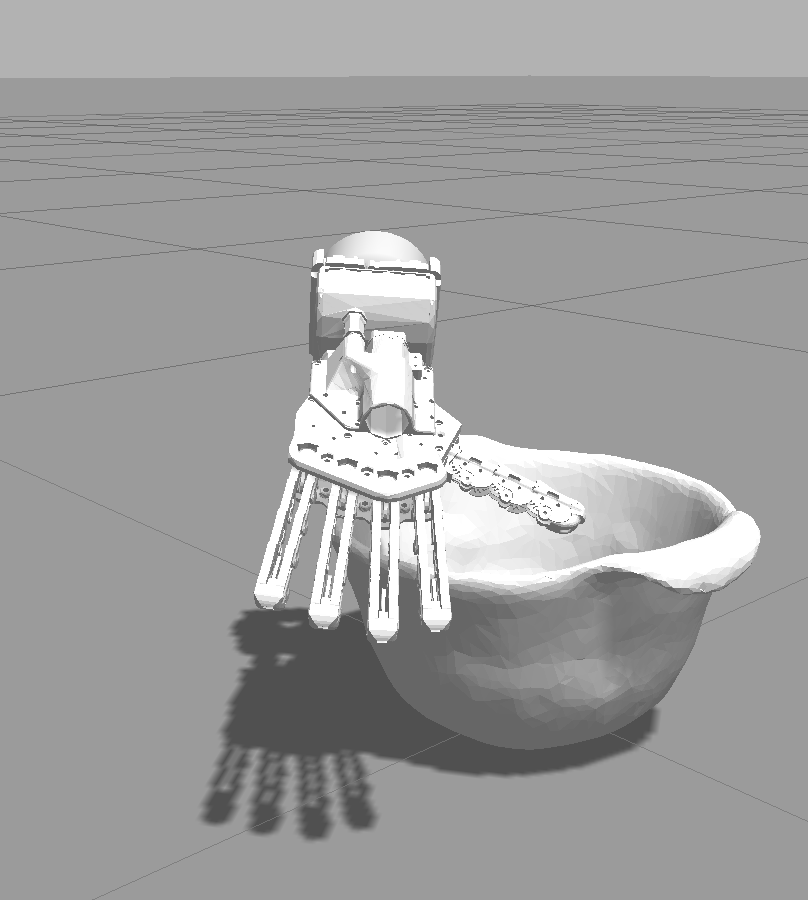
\includegraphics[width=0.3\linewidth]{containerB_pinch_2.png} &

  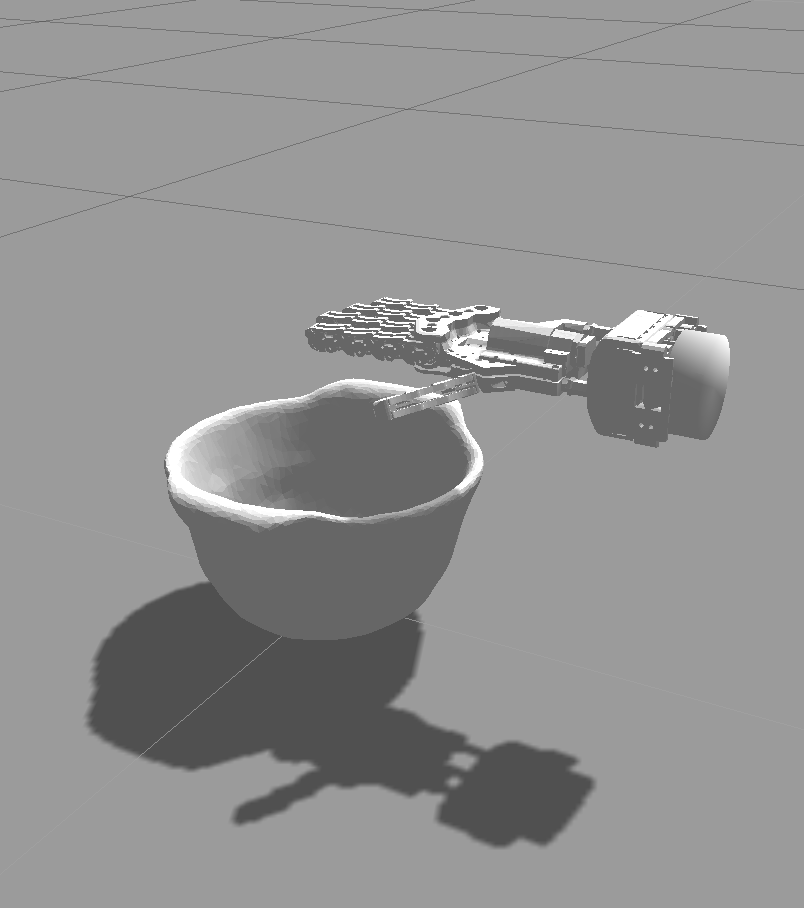
\includegraphics[width=0.3\linewidth]{containerB_rim_2.png} &

  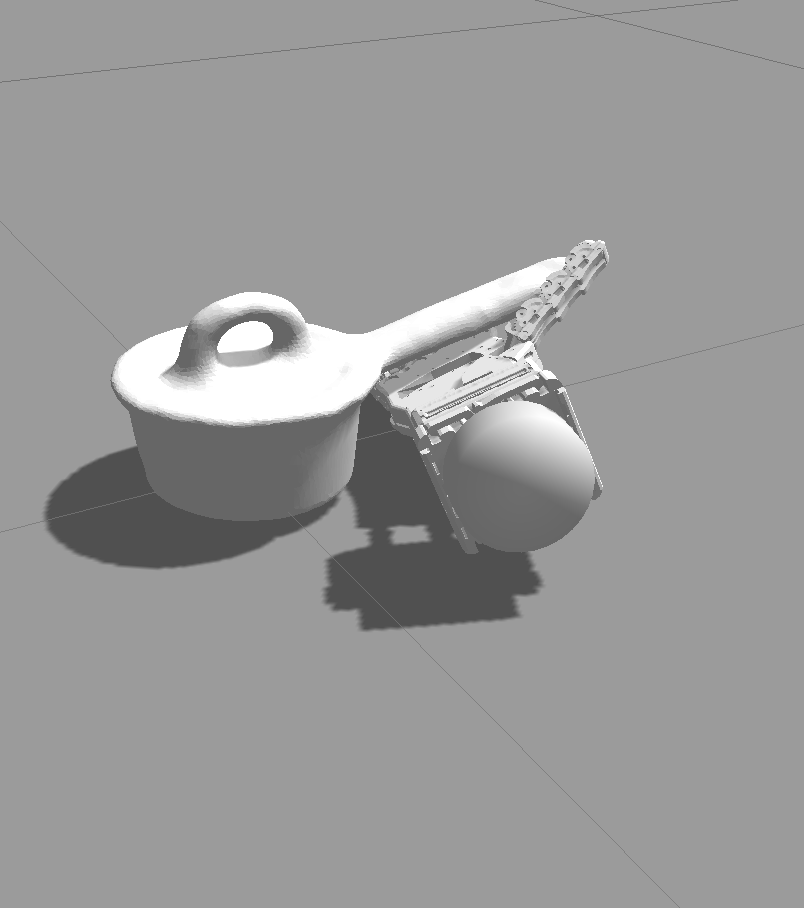
\includegraphics[width=0.3\linewidth]{pot_2.png} \\

  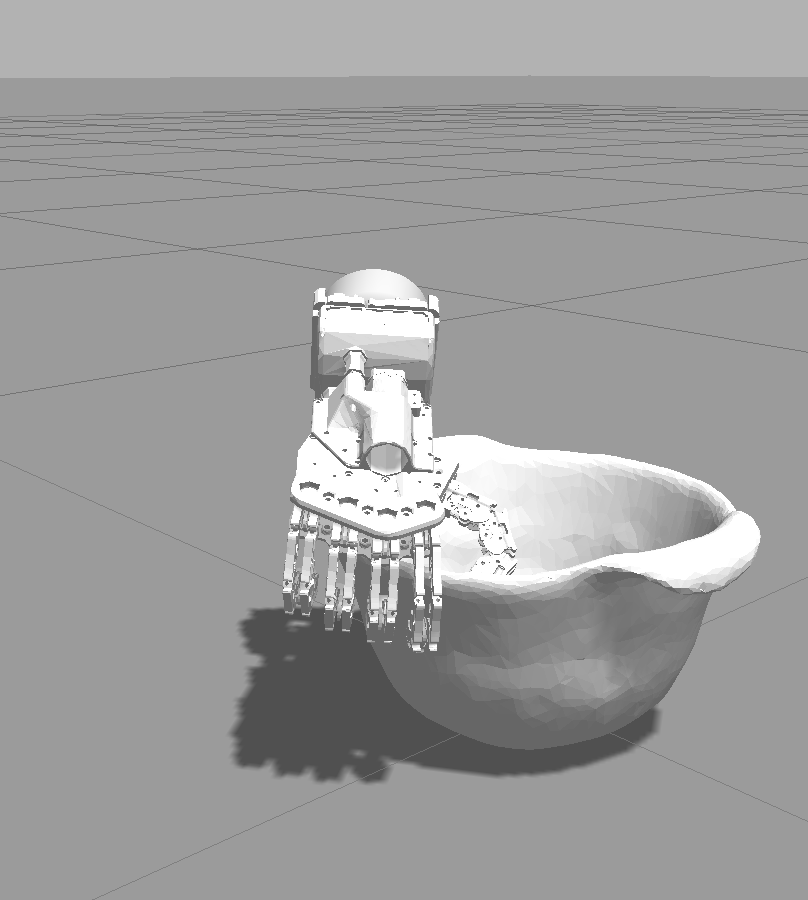
\includegraphics[width=0.3\linewidth]{containerB_pinch_4.png} &

  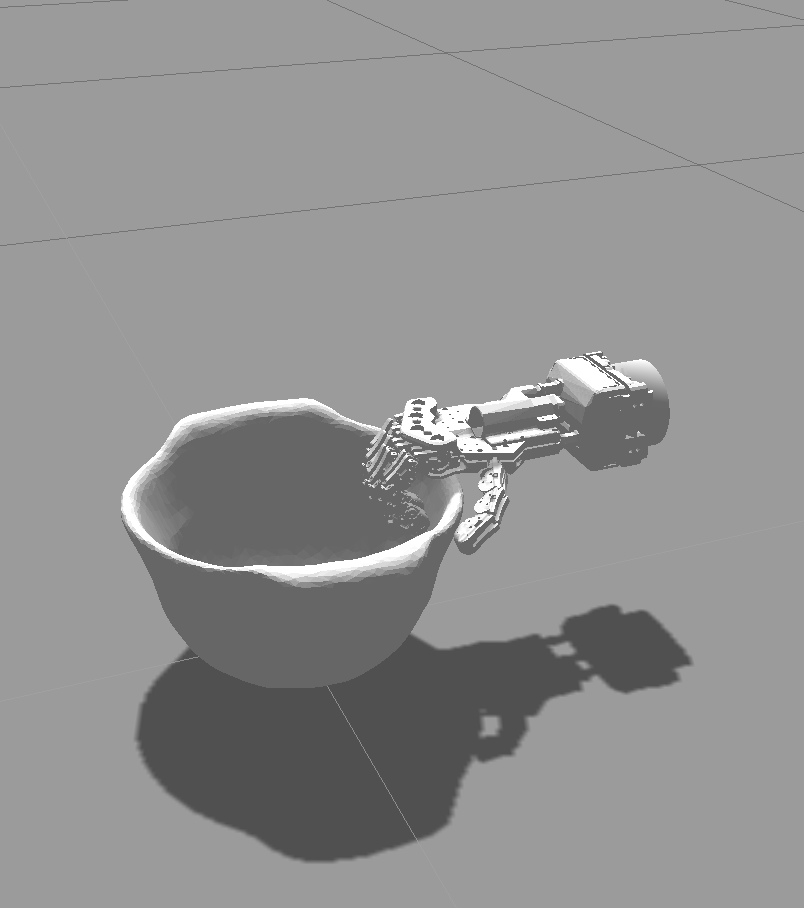
\includegraphics[width=0.3\linewidth]{containerB_rim_4.png} &

  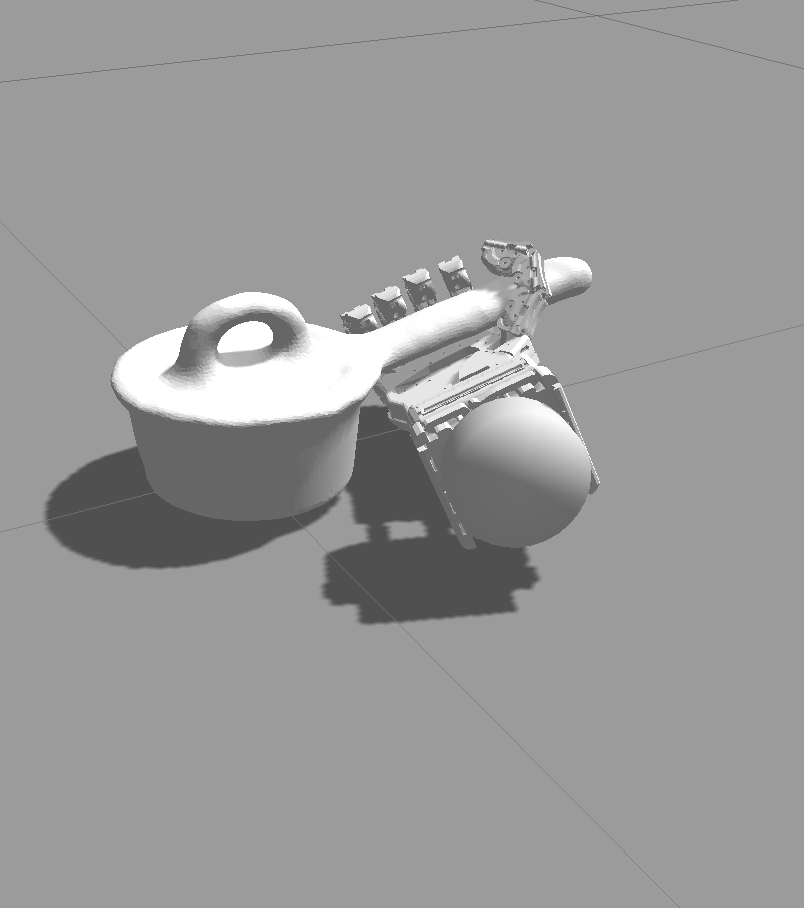
\includegraphics[width=0.3\linewidth]{pot_3.png} \\

  \end{tabular}

  \caption{Snapshots of the simulation of a pinch and rim grasp types for the colander (first and second columns), and handle grasp for the pot (last column).}
  \label{fig:simulations}
\end{figure}

%% HOW WE GENERATED THE DATA
%
At the current state, there are no generally accepted measures concerning whether a grasp by an underactuated hand  is good or not, hence the lack of robust grasp planners for them is not a surprise. Thus, generating a large dataset at this point is useless, and there are plans in the future to cover this area. As a result, we generated the examples by guiding manually the hand to a ``nice'' grasp as shown in Fig.~\ref{fig:simulations}. In this simpler scenario, we assume without loss of generality that the grasps are labelled by type. In our example dataset, we have three grasp types namely pinch, rim and by-the-handle. The main difference between pinch and rim is the fingers configuration w.r.t. the top border of objects. In the pinch grasp, the thumb goes inside whereas in the rim grasp, the fingers go inside. In the latter, the container can be filled with liquid while holding, for instance.
%
For each grasp example, the corresponding dataset comprises the set of trajectories as described in the previous section.

%For each grasp example, the corresponding dataset comprises the set of body trajectories, expicitly their position, $p_i(t) \in \mathbb{R}^3$, and orientation, $q_i(t) \in SO(3)$, over time for $i=1 , \ldots , m$ bodies (including hand links), and an associated set of hand configurations, $h_c(t) \in R^{n}$, with $n$ the hand degrees of freedom.
%%associated set of hand configurations, %$h_c(t) \in R^{n}$, with $n$ the hand degrees of freedom.

% FOR FUTURE WORK?

% Another challenge is to learn how any adaptive synergy transmission behave for any given kinematic design. 

%% BECAUSE I'M WORKING IN GENERATING DATA FOR ANOTHER COMPLIANT HAND BESIDES THE PISA SOFTHAND